\documentclass{article}
\usepackage[top=2cm,bottom=2cm,left=2cm,right=2cm]{geometry}
\usepackage{graphicx}
\usepackage{float}
\usepackage{caption}
\captionsetup{font=footnotesize}
\usepackage{booktabs}
\usepackage[super]{nth}
\usepackage{authblk}
\usepackage[normalem]{ulem}
\usepackage{orcidlink}
\usepackage{hyperref}
\usepackage{amsmath, amssymb}
\usepackage[numbers]{natbib}
\usepackage{algorithm}
\usepackage{algpseudocode}
\usepackage{graphicx}
\usepackage{subcaption}

\begin{document}

\title{PhysiGym: bridging the gap between the Gymnasium reinforcement learning application interface and the PhysiCell agent-based model software}

% ---------- Authors ----------
\author[1,2,5,$\ast$,$\dagger$]{Alexandre Bertin \orcidlink{0009-0000-7566-1979}}
\author[3,$\dagger$]{Elmar Bucher \orcidlink{0000-0002-2929-2460}}
\author[2,5]{Owen Griere}
\author[2,5]{Marcelo Hurtado \orcidlink{0009-0004-6712-0864}}
\author[3]{Heber Rocha \orcidlink{0000-0002-5876-2644}}
\author[3]{Randy Heiland \orcidlink{0000-0002-7440-2905}}
\author[3]{Aneequa Sundus \orcidlink{0000-0001-6833-2341}}
\author[3,$\ddagger$]{Paul Macklin \orcidlink{0000-0002-9925-0151}}
\author[4,$\ddagger$]{Vincent Fran\c{c}ois-Lavet \orcidlink{0000-0002-8593-9740}}
\author[1,$\ddagger$]{Emmanuel Rachelson \orcidlink{0000-0002-8559-1617}}
\author[2,5,$\ast$,$\ddagger$]{Vera Pancaldi \orcidlink{0000-0002-7433-624X}}
% ---------- Affiliations ----------
\affil[1]{CRCT, Université de Toulouse, Inserm, CNRS, Université Toulouse III-Paul Sabatier, Centre de Recherches en Cancérologie de Toulouse, France}
\affil[2]{ISAE-Supaéro, Toulouse, France}
\affil[3]{Department of Intelligent Systems Engineering, Indiana University, Bloomington, IN, USA}
\affil[4]{Department of Computer Science, VU Amsterdam, The Netherlands}
\affil[5]{Equipe Labellisée LIGUE Contre le Cancer, France}

% ---------- Contribution Notes ----------
\affil[$\ast$]{Corresponding authors: \href{mailto:alexandre.bertin@isae-supaero.fr}{alexandre.bertin@isae-supaero.fr}, \href{mailto:vera.pancaldi@inserm.fr}{vera.pancaldi@inserm.fr}}
\affil[$\dagger$]{These authors contributed equally to this work.}
\affil[$\ddagger$]{These authors contributed equally to this work.}

\date{September 16, 2025}

\maketitle
%\editor{Associate Editor: Name}

%\abstract{
%\textbf{Motivation:} .\\
%\textbf{Results:} .\\
%\textbf{Availability:} .\\
%\textbf{Contact:} \href{name@email.com}{name@email.com}\\
%\textbf{Supplementary information:} Supplementary data are available at \textit{Journal Name}
%online.}

\abstract{
This paper presents PhysiGym, a framework that integrates agent-based biological simulation within standardized reinforcement learning environments. 
By integrating the agent-based modeling framework PhysiCell with the Gymnasium API, we provide a flexible tool for exploring reinforcement learning strategies to control in-silico biological processes. 
We demonstrate PhysiGym's potential with a case study where a deep reinforcement learning algorithm guides a tumor microenvironment model toward an anti-tumoral state, ultimately achieving tumour elimination. 
Our results highlight PhysiGym's flexibility for AI-driven biological control and optimization of dynamic treatment regimes.
%Our results demonstrate that PhysiGym provides a flexible framework for AI-driven biological control, allowing adaptive strategies to regulate complex biological systems.
}

\maketitle
\section{Introduction}
Biological systems are complex, dynamic, and often difficult to study in real life. 
In silico modeling aims to mimic these systems, providing a controlled environment for exploring specific aspects of biological processes and testing hypotheses.
In particular, agent-based models (ABMs) provide a powerful framework for simulating biological systems where agents (e.g. cells) interact dynamically based on predefined rules. These models are used in oncology and immunology  to study emerging behaviors in complex biological systems, with the potential to propose novel therapeutic strategies \citep{johnson2023digitize, laubenbacher2024toward, rocha2024multiscale}.

Ordinary differential equations (ODEs) and agent-based models (ABMs) are widely used to simulate the tumor microenvironment (TME). ODEs provide compact system-level descriptions, while ABMs capture spatial and cellular heterogeneity at higher computational cost. For dynamic treatment regimes (DTRs) \citep{gray1982arac}, however, simulation alone is insufficient: designing adaptive, sequential interventions requires a control framework. Reinforcement learning (RL), where an RL agent learns policies through interaction with an environment, offers such a framework~\citep{barto1989learning}. By modeling treatment regimes as a sequence of decisions, RL enables adaptive control of biological simulations~\citep{chakraborty2014dynamic}. For efficient experimentation and policy learning, RL further requires a standardized interface. To address this, we introduce PhysiGym, an interface that connects PhysiCell \citep{ghaffarizadeh2018physicell}, an ABM framework for multicellular simulations of tissues or cell cultures (tumor microenvironment, other disease tissues, or bacteria colonies), with Gymnasium \citep{towers2024gymnasium}, a widely adopted RL application programming interface (API). 
PhysiCell enables flexible multiscale modeling of biological systems, coupled with a sophisticated underlying physics simulator (the BioFVM  diffusion transport solver \citep{ghaffarizadeh2016biofvm}), while Gymnasium provides a structured framework for training and evaluating RL policies.

The first implementation of RL on an ABM framework based on BioFVM was proposed by \citet{zade2020reinforcement}, which applied Q-learning \citep{watkins1992q} to optimize Temozolomide treatment regimes for patients with glioblastoma multiforme, a highly specific problem. 
More recently, \citet{aif2025failing} used PhysiCell as a complex (high-fidelity) simulation environment for tumor growth, combined with a simple (low-fidelity) RL training environment of coupled ordinary differential equations (ODE)  to learn treatment strategies for solid tumors.


PhysiGym bridges PhysiCell and Gymnasium to provide a reproducible and scalable framework for integrating agent-based simulations of biological systems with RL strategies. In the following, we present PhysiGym’s motivation and design, demonstrating how it directly connects ABMs and RL to control complex biological systems. In particular, we focus on the tumor microenvironment, a biological system made up of cancer cells and surrounding immune and stromal cells that engage in complex interactions and cross-talks, which is proven to be crucial for an effective response to immunotherapy, an important therapeutic approach in an increasing number of types of cancer. 
% BUE additionally, maybe:                                             
% Physicell version 1.14.2, released in January 2025, implemented by us — it was not possible to run a series of episodes of a model in a single runtime, which is indispensable for DL and RL. 
\section{Methods}
% instead of 
\subsection{PhysiGym design and implementation}\label{sec2}
PhysiCell is an ABM framework written in C++ and implemented to model multicellular systems based on classical mechanics  \citep{ghaffarizadeh2018physicell}. Cells are agents whose type determines the specific rule set that governs their behavior and interactions with the other agents and the environment. Substrates, like oxygen or cytokines, can be modeled with the integrated BioFVM diffusive transport solver \citep{ghaffarizadeh2016biofvm}. In addition, intracellular models can be integrated into cell agents \citep{letort2018physiboss, ponce2023physiboss, ruscone2024physiboss} to model specific behaviors based on each cell's environment and gene regulatory networks. The extracellular matrix that surrounds cells in tissues can also be modeled as a mesh of fibers for a more realistic representation of the cells' physical environment \citep{noel2024physimess}. 
Together, these components enable the construction of ABMs that are spatially explicit in two or three dimensions, off-lattice, center-based, and multiscale in both space and time \citep{metzcar2019review}. 

RL is used to control discrete-time dynamical systems, which are typically modeled as Markov Decision Processes (MDPs) \citep{bellman1957markovian, puterman2014markov}. 
An MDP consists of four key elements:
\begin{enumerate}
    \item $S$ the state space, where $s\in S$ represents a state of the environment.
    \item $A$ the action space, where $a \in A$ represents an action applied to the environment (e.g. drug dose).
    \item $T$ the transition model, which defines how the environment evolves. The transition model can be either deterministic or stochastic. Formally, the next state noted $s'$ is given by $s'\sim T(s,a)$ where $s$ represents the current state and $a$ the action taken.
    \item $R$ the reward function, which evaluates whether an action was beneficial. Formally, $r$ denotes the reward obtained by taking action $a$ in state $s$, i.e., $r = R(s,a)$.
\end{enumerate}
The objective is to find the policy that maximizes the expected discounted cumulative reward:
$$
\underset{\pi\in\Pi}{\arg\max} \ \mathbb{E} \left[ \sum_{t=0}^{\tau} \gamma^t r_t \mid s_0 = s, \pi \right],
$$
with $s_0$ the initial state, $\pi$ the policy, $\gamma$ the discount factor, and $\tau$ the terminal timestep.
In the RL community, the Gymnasium RL API is widely used as a standard interface for MDPs, promoting code reuse and modularity in RL algorithms and models.

PhysiGym bridges the gap between the PhysiCell ABM framework and the Gymnasium RL API by extending the Python interpreter \citep{rossum1995extending, psf2024extending} with PhysiCell. As a result, the ABM model is implemented in the same way as standard PhysiCell models, using PhysiCell Studio \citep{heiland2024physicellstudio} and C++.  

Any model implemented in PhysiCell can be converted into a PhysiGym model. 
The interface between PhysiCell and Gymnasium is based on the PhysiCell "user parameter", "custom data variable", and "custom data vectors" data constructs. Information, such as how much drugs to apply to the domain, can only be transferred over these variable types. The variables (for example, drug) can easily be specified in PhysiCell Studio under the \texttt{User Params} and \texttt{Cell Types / Custom Data} tab.
As a minimum requirement, the user must define the parameter $dt\_gym$, which specifies the time interval at which interactions with the environment occur, and the parameter $time$, a time tracker necessary to determine when to update the environment.
In addition, additional parameters can be defined to control the simulation, such as drug administration, which can serve as actions. Similarly, other parameters can be designated to record specific quantities of interest, which can then be used to construct the observations.

According to the transition function, for each episode (a complete sequence of states, actions, and rewards from the start to the end of a trial), values from these data constructs can be modified without having to recompile the source code.
There are three additional functions to define the state space (read information from the simulation): \texttt{get\_cell} for cell position, \texttt{get\_microenv} for substrate concentration, and \texttt{get\_graph} to retrieve cell neighborhood information. 

To extend the Python interpreter with PhysiCell, the main simulation loop, written in C++, was split into three functions: \texttt{physicell\_start}, \texttt{physicell\_step}, and \texttt{physicell\_stop}, all of which can be called from Python. 
The \texttt{physicell\_start} function initializes the PhysiCell model, while \texttt{physicell\_stop} terminates the simulation. 
The \texttt{physicell\_step} function is responsible for advancing the environment by one time step based on the action taken by the reinforcement learning agent.
For most models, only \texttt{physicell\_step} needs to be modified, e.g. to apply drugs to the ABM.
Several additional C++ functions are exposed in Python to facilitate data retrieval.
These include functions to obtain custom variables, vectors, \texttt{physicell\_get\_cell}, which provides a matrix containing information about each cell, such as its type, coordinates, and death status, and \texttt{physicell\_get\_microenv}.
All exposed functions are implemented in the C++ file \texttt{physicellmodule.cpp}.

By extending the necessary functions to obtain the desired control over the ABM and modifying the \texttt{physicell\_step} function, users can compile the C++ code and integrate it with Python, particularly with the Gymnasium API. This allows users to define \texttt{physicell\_model.py}, which implements a Gymnasium-compatible environment. Specifically, \texttt{physicell\_model.py} defines a child class of Gymnasium’s environment class, inheriting from \texttt{CorePhysiCellEnv} which is specified in \texttt{physicell\_core.py}.
\texttt{CorePhysiCellEnv} is the main class that takes charge of the use of \texttt{physicell\_start}, \texttt{physicell\_stop} and \texttt{physicell\_step} which are model independent.
This class handles interactions with the Gymnasium framework. 
Users should modify \texttt{physicell\_model.py} to specify the observation space, action spaces, and the reward, as well as any additional data they wish to store.

For more details, consult the reference manual \url{https://github.com/Dante-Berth/PhysiGym/blob/main/man/REFERENCE.md}.

For an in-depth understanding, tutorials are provided and can be found at the PhysiGym GitHub home page.
Besides, pytest unit tests are included in the code base, and we use GitHub Actions for continuous integration.
%These tests help ensure that the code remains functional when new features are added or updates are made, preventing any potential inconsistencies. 
PhysiGym was extensively tested for compiling and running on Linux, Windows Subsystem for Linux, and macOS. 
Installation and troubleshooting how-tos, a modeling tutorial, an RL tutorial, and a reference manual can be found at [\url{https://github.com/Dante-Berth/PhysiGym/tree/main/man}].


\subsection{Implementation of a tumor microenvironment toy model \ref{ToyModel}}

We developed a simplified tumor microenvironment (TME) model \ref{ToyModel} to illustrate the potential uses of PhysiGym. The model includes four cell types, four diffusible substrates, and a set of simple agent-based rules.
At the initial state, the total number of \texttt{tumor} cells is 512. And 128 \texttt{cell\_1} surrounds the tumor.
Moreover the total number of \texttt{cell\_1} and \texttt{cell\_2} is fixed at 128. 
\subsubsection*{1. Cell types}

\begin{itemize}
  \item \textbf{Tumor cells}: proliferate ($5 \times 10^{-5} \, \text{min}^{-1}$), apoptosis ($1 \times 10^{-6} \, \text{min}^{-1}$), immotile, uptake anti- and pro-tumoral factors. Necrosis, motility, and baseline secretion disabled.
  \item \textbf{Cell\_1}: non-proliferative, mobile, uptakes pro-tumoral factor ($10/\text{min}$). Conditional rules allow secretion of anti-tumoral factor and transformation into cell\_2.
  \item \textbf{Cell\_2}: non-proliferative, mobile, uptakes drug\_1 ($10/\text{min}$), produces pro-tumoral. Conditional rules allow transformation into cell\_1 in presence of drug\_1.
\end{itemize}

\subsubsection*{2. Substrates}

\begin{enumerate}
  \item \textbf{Debris}: produced by dead tumor cells, diffusion $1 \, \mu m^2/\text{min}$, no decay. Acts as a signal for debris-related rules.
  \item \textbf{Drug\_1}: decay $0.01/\text{min}$, applied at boundaries, regulates \texttt{cell\_2} $\rightarrow$ \texttt{cell\_1} transformation.
  \item \textbf{Anti-tumoral factor/ pro-inflammatory factor}: diffusion $1000 \, \mu m^2/\text{min}$, decay $0.05/\text{min}$, secreted conditionally by \texttt{cell\_1}, enhances tumor apoptosis.
  \item \textbf{Pro-tumoral factor/ anti-inflammatory factor}: diffusion $1000 \, \mu m^2/\text{min}$, decay $0.1/\text{min}$, is  produced by \texttt{cell\_2} and enhances tumor survival.
\end{enumerate}

\subsubsection*{3. Cell Hypothesis Rules}

In \texttt{tumor} cells: pressure decreases cycle entry from 5e-05 towards 0 with a Hill response, with half-max 5 and Hill power 3.
pressure increases necrosis from 0 towards 0.0028 with a Hill response, with half-max 10 and Hill power 3.
anti-inflammatory factor decreases apoptosis from 1e-06 towards 0 with a Hill response, with half-max 5 and Hill power 10.
pro-inflammatory factor increases apoptosis from 1e-06 towards 0.05 with a Hill response, with half-max 1 and Hill power 2.
dead increases debris secretion from 0 towards 0.25 with a Hill response, with half-max 0.2 and Hill power 5. Rule applies to dead cells.

In \texttt{cell\_1} cells: pressure increases transform to \texttt{cell\_2} from 0 towards 1 with a Hill response, with half-max 11 and Hill power 4.
anti-inflammatory factor decreases pro-inflammatory factor secretion from 10 towards 0 with a Hill response, with half-max 10 and Hill power 4.

In \texttt{cell\_2} cells: \texttt{drug\_1} increases transform to \texttt{cell\_1} from 0 towards 1 with a Hill response, with half-max 5 and Hill power 4.


This toy model highlights how the RL framework can control tumor progression by modulating the whole microenvironment, rather than solely targeting cancer cell killing.


\begin{figure}[h]%
\centering
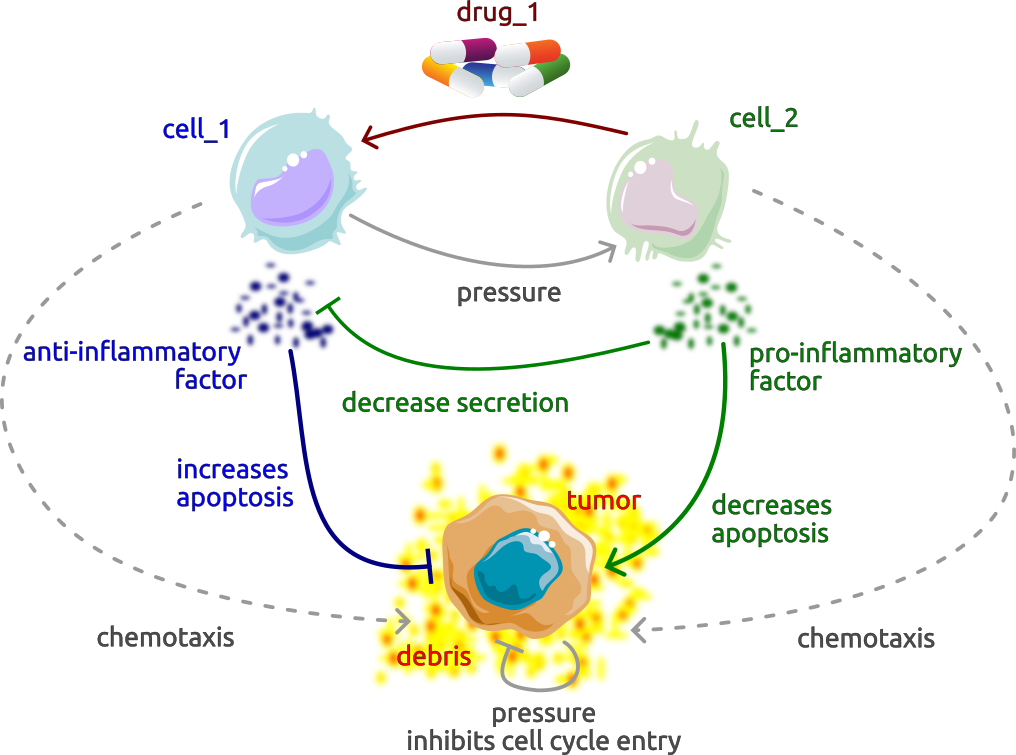
\includegraphics[width=0.7\textwidth]{img/model_tumor_immune_base.png}
\caption{Toy model of the tumor microenvironment, representing interactions between cancer cells and two  other distinct cell types with specific behaviors, together with exchanged cytokines and different processes. $\dashv$ represents an inhibition, while $\rightarrow$ represents an activation. The color of the arrows corresponds to the color of the cell producing the protein associated with the arrow. For instance, \textbf{cell\_1} is in blue; thus, the arrow related to increasing apoptosis of the tumor is also in blue, as in \textbf{cell\_1}.}
\label{ToyModel}
\end{figure}

\subsection{Implementation of an RL approach to control the TME simulation}

% We begin with S the state, explain the different states, then going to A the action , one comment to T and finally finish with the reward noted R
Our overall objective is to achieve complete tumor eradication while minimizing drug exposure and avoiding aggressive dosage escalation.
\subsection{State space $S$}
In an tumor microenvironment, they are different type of cells, but also different molecules/ chemical compounds view as substrates. Besides, it exists different type of data, data which gives an inisght on the space and others data are spaceless such as a simple vector comporting some stastics about the tumor micro environment. Overall, we propose to study in this model the importance of different state space on dynamic treatment regime in order to compare them on multiple metrics such as the cumulative return.
The simulator provides multiple data, given that we can build different state spaces, we have considered scalars, images and graphs. We could ask, state space related to are superior to simple scalars related to space. 
We propose multiple different observation spaces, depending on whether we consider the spatial aspect of the simulation or not.
\subsubsection{Scalars Observation Spaces}
 We denote by $\text{cell}_i(t)$ the number of cells of type $i$, with $i \in \{0,1,2\}$. Where $\text{cell}_1(t=0)$ refers to the number of tumor cells at the initial time, in our case it equals to 512. We use this term, to normalize any cell numbers.
 Let $\mathcal{T}$ denote the set of cell types and $|\mathcal{T}| = N_c$.
 Let $\mathcal{S}$ be the set of substrates with $|\mathcal{S}| = N_s$, in particularly $\mathcal{S} = \{\text{debris}, \text{anti-inflammatory factor}, \text{pro-inflammatory factor}, \text{drug}_1\}$
 Besides, we denote $sub_{j,t}$ as the amount of the substrate in the entire environment thus $sub_{j,t}\in (R^{+})^{width*height}$
 
\paragraph{Scalar Cell Counts (\texttt{scalars\_cells}).}
This observation space consists only of normalized cell counts for each cell type.
For each cell type $i \in \mathcal{T}$, we compute
$$
s^{\text{cells}}_i(t) = \frac{\text{cell}_i(t)}{c_{\text{init}}} - 1,
$$
where $c_{\text{init}}$ is the initial number of cancer cells.
The resulting observation vector is
$$
s_t^{\text{cells}} \in \mathbb{R}^{N_c}.
$$

\paragraph{Scalar Substrate Values (\texttt{scalars\_substrates}).}
This observation space captures only the maximum concentration of each substrate over the entire spatial domain.
For each substrate $j \in \mathcal{S}$, we define
$$
s^{\text{sub}}_j(t) = \max\left(sub_{j,t}\right),
$$
where $sub_{j,t}$ denotes the spatial field of substrate $j$ at time $t$.
The observation is then
$$
s_t^{\text{sub}} \in \mathbb{R}^{N_s}.
$$

\paragraph{Scalar Cells and Substrates (\texttt{scalars\_cells\_substrates}).}
This representation concatenates the two previous scalar observations:
$$
s_t^{\text{cells+sub}} =
\left(
s_t^{\text{cells}},\;
s_t^{\text{sub}}
\right)
\in \mathbb{R}^{N_c + N_s}.

$$

\subsubsection{Image-Based Observation Spaces}

We consider the spatial distribution of cells and substrates via an image representation of the simulation state. A set of channels corresponds to a specific cell type, while the other set of channels refers to the substrates. Substrates are chemical products or extracellular proteins produced by cells or produced by the environment or chemical products added to the environment, such as drugs. To reduce memory requirements, we reduce the shape of the original image given by the \texttt{PhysiCell\_Settings.xml} file by discretizing the continuous environment onto a uniform grid. We also compute $g_{x}=\lfloor \frac{width}{gridsize_{x}}\rfloor$ and $r_{y}=\lfloor\frac{height}{gridsize_{y}}\rfloor$. In our environment, $g_{x}=g_{y}$ because $width = height = 512$ and $gridsize_{x}=gridsize_{y}=gridsize=64$.
The size of the bins is calculated by mapping the continuous coordinates into discrete indices. Specifically:

$$
x_{\text{bin}} = \left\lfloor 
\frac{(x - x_{\min})}{(x_{\max} - x_{\min})}
\times (gridsize_{x} - 1)
\right\rfloor,
$$
$$
y_{\text{bin}} = \left\lfloor 
\frac{(y - y_{\min})}{(y_{\max} - y_{\min})}
\times (gridsize_{y} - 1)
\right\rfloor.
$$
This ensures that the continuous spatial domain is discretized into a grid of size 
\(gridsize \times gridsize\).
If one or more cells are present in a bin, we increment the count in the channel corresponding to the respective cell type. Formally, for each cell:
\begin{itemize}
    \item Determine its bin index $(x_{\text{bin}}, y_{\text{bin}})$.
    \item Increment $\text{image}[c, y_{\text{bin}}, x_{\text{bin}}]$ by $\frac{1}{r_x r_y}$.
\end{itemize}

By dividing by $g_{x}g_{y}$, we normalize the count so that the value in each bin represents an area contribution, ensuring that our image values stay in the range $[0,1]$.
This produces an image tensor of shape $(\text{num cell types}, gridsize, gridsize)$,
Thus, for our three cell types, we can represent the data by images, as shown in figure \ref{spatialchannels}.

\begin{figure}[h!]%
\centering
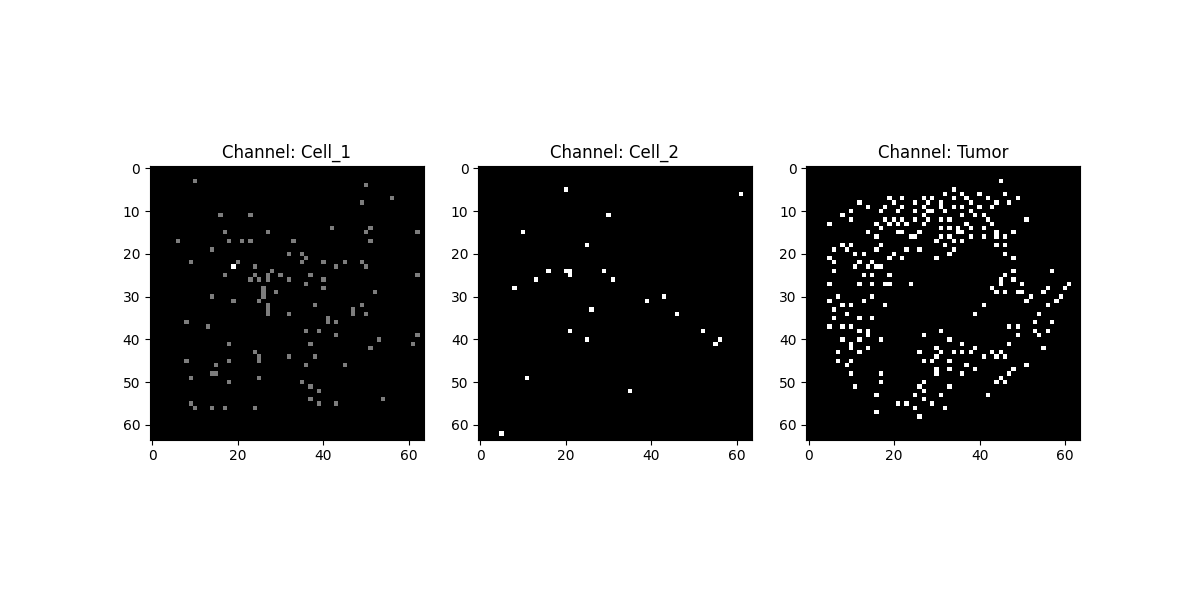
\includegraphics[width=1.0\textwidth]{img/image_cell_types.png}
\caption{Representation of different channels, each channel represents a cell type.}
\label{spatialchannels}
\end{figure}
For substrate channels, the process is similar but simpler, since substrate values are continuous. Using the same $(x_{\text{bin}}, y_{\text{bin}})$ discretizations, we assign each bin the maximum substrate value observed in that bin. A min-max normalization is then applied across the entire image for each substrate channel, bringing all values into range $[0, 1]$, which can be seen in figure~\ref{spatialchannelssubstrates}.

\begin{figure}[h!]%
\centering
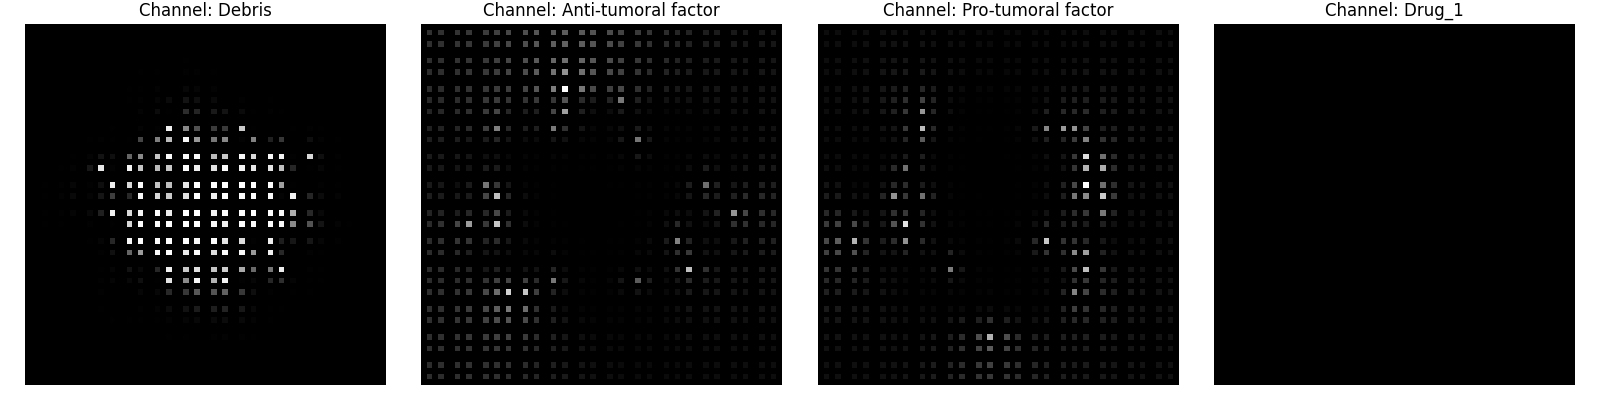
\includegraphics[width=1.0\textwidth]{img/img_substrates.png}
\caption{Representation of different channels; each channel represents a substrate.}
\label{spatialchannelssubstrates}
\end{figure}

\paragraph{Multi-Channel Cell Images (\texttt{img\_mc\_cells}).}
This observation space extends the spatial discretization described earlier by encoding each cell type into a separate image channel.
After discretization, the image tensor is
$$
s_t^{\text{mc-cells}} \in \mathbb{N}^{N_c \times g_x \times g_y},
$$
where each channel represents the normalized spatial density of one cell type, rescaled to the range $[0,255]$.

\paragraph{Multi-Channel Substrate Images (\texttt{img\_mc\_substrates}).}
Similarly, each substrate is represented as a separate image channel.
For each grid cell, the maximum substrate concentration observed in that bin is assigned.
A min--max normalization is applied independently to each substrate channel:
$$
\tilde{s}_{j}(x,y) =
\frac{s_{j}(x,y) - \min s_{j}}{\max s_{j} - \min s_{j}},
$$
yielding an image tensor
$$
s_t^{\text{mc-sub}} \in \mathbb{N}^{N_s \times g_x \times g_y}.
$$

\paragraph{Multi-Channel Cells and Substrates (\texttt{img\_mc\_cells\_substrates}).}
This observation space concatenates the cell and substrate image channels along the channel dimension:
$$
s_t^{\text{mc-cells+sub}} \in \mathbb{N}^{(N_c + N_s) \times g_x \times g_y}.
$$

\subsubsection{Graph-Based Observation Spaces}

\paragraph{Cell Interaction Graphs (\texttt{graph\_delaunay} and \texttt{graph\_knn}).}
In these observation spaces, the cellular population is represented as a graph
$$
\mathcal{G}_t = (\mathcal{V}_t, \mathcal{E}_t),
$$
where each node $v \in \mathcal{V}_t$ corresponds to a living cell, and edges are constructed either via Delaunay triangulation or $k$-nearest neighbors in the $(x,y)$ plane.

Each node is associated with a feature vector
$$
\mathbf{x}_v = \frac{\text{type}(v)}{N_c},
$$
encoding the normalized cell type.
Each edge $(u,v) \in \mathcal{E}_t$ carries a scalar attribute corresponding to the normalized Euclidean distance between the two cells:
$$
\mathbf{e}_{uv} = \frac{\lVert \mathbf{p}_u - \mathbf{p}_v \rVert}{\max(\text{width}, \text{height}, \text{depth})}.
$$

To allow batching, graphs are padded to fixed sizes with $N_{\max}$ nodes and $E_{\max}$ edges.
Binary masks indicate valid nodes and edges.
The final observation is given by the tuple
$$
s_t^{\text{graph}} =
\left(
\mathbf{X},\;
\mathbf{E},\;
\mathbf{A},\;
\mathbf{m}_V,\;
\mathbf{m}_E
\right),
$$
where $\mathbf{X} \in \mathbb{R}^{N_{\max} \times d_V}$ are node features,
$\mathbf{A} \in \mathbb{N}^{2 \times E_{\max}}$ is the edge index tensor,
$\mathbf{E} \in \mathbb{R}^{E_{\max} \times d_E}$ are edge attributes,
and $\mathbf{m}_V$, $\mathbf{m}_E$ are node and edge masks, respectively.

\subsection{Action $A$ $\&$ Reward $R$}
In reinforcement learning, the reward function plays a central role, as it provides the learning signal that links actions to their long-term consequences on the environment. An inadequately designed reward may lead to misleading gradients and suboptimal or unstable policies, even when the state and action spaces are well defined. In our setting, reward design is particularly critical, as the objective involves a delicate trade-off between reducing tumor burden and limiting the amount of drug introduced into the tumor microenvironment.

In the literature, numerous reward or cost formulations have been proposed for chemotherapy scheduling and related clinical control problems. Many works in optimal control and clinical reinforcement learning define the objective as a combination of disease burden and treatment cost. Classical optimal control studies consider objectives of the form.

Many works in optimal chemotherapy scheduling and clinical reinforcement learning formulate the reward or cost function as a combination of disease burden and treatment cost. Classical optimal control studies use objectives of the form  $\int_0^T (w_1 C(t) + w_2 u(t))\,dt$,  with $C(t)$ denoting tumor size and $u(t)$ the administered drug, to balance tumor reduction and toxicity  \cite{ledzewicz2016drug}. In reinforcement learning settings, similar  formulations appear in the context of adaptive dosing, including $r_t = -C_t - \alpha u_t$ for chemotherapy and analogous expressions in sepsis management \cite{raghu2017deep}. In this work, we propose a novel reward formulation that extends this paradigm by normalizing tumor response relative to the expected untreated growth and by introducing an explicit penalty on dosage escalation, thereby capturing both cumulative exposure and toxicity associated with abrupt increases in drug administration.

At each control step $t$, the agent selects a drug administration action
$$
u_t \in [0,1],
$$
where $u_t = 0$ corresponds to no drug administration and $u_t = 1$ corresponds to the maximum admissible drug concentration applied to the tumor microenvironment.
The action space is therefore defined as:
$$
A = [0,1].
$$

Let $c_t$ denote the total number of tumor cells at time $t$.
For our basic model and in the absence of treatment, tumor growth is assumed  to follow an exponential model \cite{watanabe2016mathematical}:
$$
\frac{dc(t)}{dt} = \lambda c(t),
$$
We can derivate an expected untreated tumor growth over one control interval $\Delta t$:
$$
\Delta c_t^{\mathrm{exp}} = c_t \left( e^{\lambda \Delta t} - 1 \right).
$$
We used this term as a normalizing factor $\Delta c_t^{\mathrm{exp}}$.
We can define a normalized tumor growth:
$$
r_{\mathrm{tumor}}(t)
=
\frac{c_t - c_{t+\Delta t}}{\Delta c_t^{\mathrm{exp}}},
$$
which measures the reduction in tumor size relative to its expected natural growth.
The tumor growth rate $\lambda$ is computed as
$$
\lambda = \text{cycle} \ln(2) - d ,
$$
where the parameters are specified in \texttt{PhysiCell\_Settings.xml}.  
Here, $\text{cycle}\in R^{+}$ denotes the cell-cycle transition rate (division rate), and $d\in R^{+}$ denotes the cell death rate.



In addition to tumor suppression, drug usage is penalized by the mean administered dose:
$$
r_{\mathrm{amount}}(t) = u_t,
$$
and an additional penalty is introduced for dosage escalation between consecutive time steps:
$$
r_{\mathrm{increase}}(t) = \max(0, u_t - u_{t-1}).
$$

The final reward function is defined as:
$$
r_t
=
w_{tumor} \, r_{tumor}(t)
-
w_{amount} \, r_{amount}(t)
-
w_{increase} \, r_{increase}(t),
$$
where $w_{tumor}, w_{amount}, w_{increase} \ge 0$ are weighting coefficients satisfying:
$$
w_{tumor} + w_{amount} + w_{increase} = 1.
$$
The values of weights are: $w_{tumor} = 0.7$, $w_{increase}=0.2$, $w_{amount}=0.1$. The weight $w_{tumor}$ controls the tumor eradication, while $w_{amount}$ and $w_{increase}$ regulate overall drug exposure and temporal smoothness of the treatment protocol, respectively.
Increasing $w_{tumor}$ prioritizes tumor suppression at the cost of higher drug administration, whereas increasing $w_{amount}$ or $w_{increase}$ encourages more conservative dosing strategies.
Importantly, the proposed reward formulation is generic and reusable.
It does not introduce environment-specific hyperparameters that require tuning for stability or convergence.
Instead, the weights reflect only the user’s therapeutic preference between tumor control and drug toxicity.
As a result, this reward remains robust across different temporal resolutions and modeling assumptions,
while consistently encouraging both tumor reduction and minimized drug administration.




To address our control objective maximizing cancer cell eradication while minimizing drug administration we employ Soft Actor-Critic (SAC) \citep{haarnoja2018soft}, a state-of-the-art reinforcement learning algorithm for continuous control. SAC is particularly well suited to our setting due to its high sample efficiency, enabling effective learning from a limited number of environment interactions. Moreover, as a deep reinforcement learning method, SAC  accommodates different observation types, such as image-based representations, through the use of Convolutional Neural Networks (CNN)  \citep{o2015introduction} or graphs by the use of Graph Neural Networks (GNN)\cite{scarselli2008graph}.

A key challenge in our work is the computational cost of the simulator. To alleviate this bottleneck, we adopt an asynchronous parallel training framework inspired by \citet{mnih2016asynchronous}, and specifically leverage the Asynchronous SAC formulation introduced in \citet{liu2025asynchronous}. 

In this framework, multiple environments are executed concurrently using a decoupled architecture. A dedicated learning process performs policy and value updates on the GPU, while multiple environment processes run in parallel on the CPU to generate experience. These processes operate continuously and asynchronously, without global synchronization, enabling efficient utilization of computational resources.

\begin{figure}[h!]%
\centering
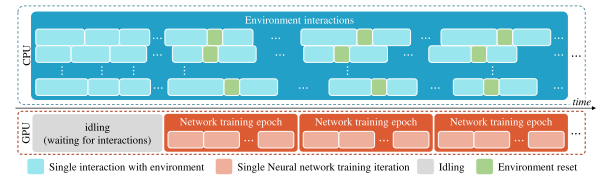
\includegraphics[width=1.0\textwidth]{img/APT.png}
\caption{ Asynchronous parallel training figure from \cite{liu2025asynchronous}
}
\end{figure}





\section{Results}
In our experimental evaluation, we compare multiple state-space representations with the hyperparameters of the Asynchronous SAC algorithm fixed as described in Table~\ref{tab:rl_hyperparameters}.
As demonstrated in Figure~\ref{performance}, we observe at the beginning learning possible faster for scalars state space but around  $0.75 \times 10^{5}$ training steps we observe than graph and image state spaces are superior to scalars state space in terms of return and around $1.00 \times 10^{5}$. In terms of sample efficiency, state spaces related to space are more sample efficient than scalars state space.
\begin{figure}[h!]%
\centering
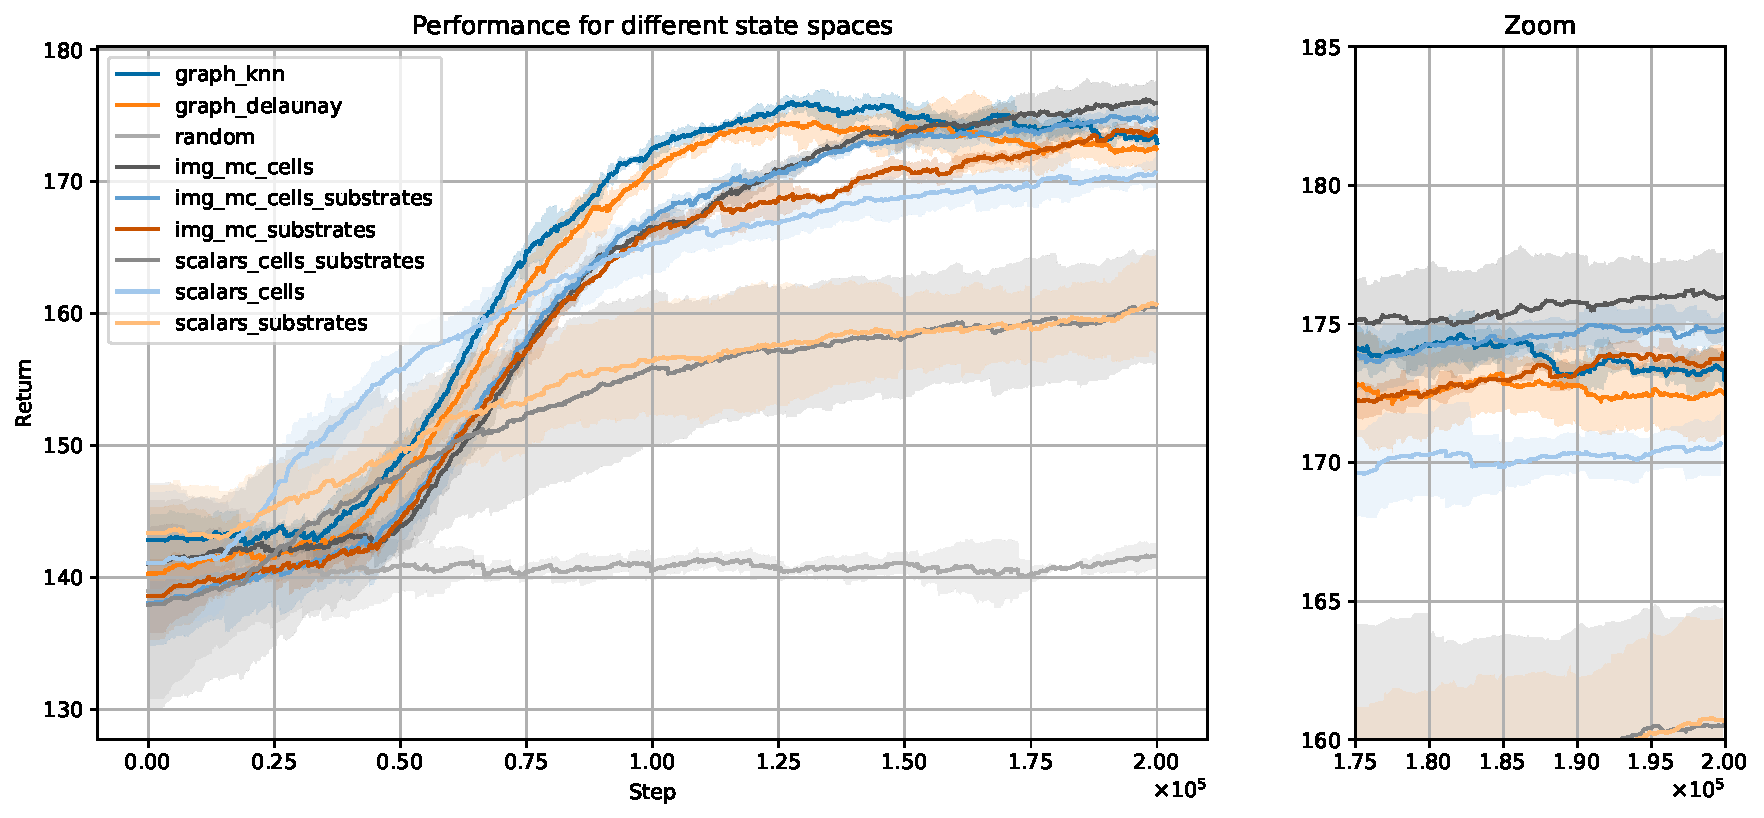
\includegraphics[width=1.0\textwidth]{img/performance}
\caption{Performance for different state spaces X-axis represents the number of steps while Y-axis represents the return across 5 different seeds.}
\label{performance}
\end{figure}



\begin{table}[htbp]
\centering
\caption{Final performance metrics for different observation modalities. Values are reported at the final evaluation step as mean ($\mu$), standard deviation ($\mu$) and relative variation noted $\%$ (computed according to: $\frac{\mu_{observation\_type} - \mu_{random}}{\mu_{random}}$)}
\label{tab:obs_type_results}
\begin{tabular}{lcccc}
\hline
\textbf{Observation type} &
\textbf{$\mu$} &
\textbf{$\sigma$} &
\textbf{$\%$}\\
\hline
Random &
141.63 &
0.94 &
0.0 \\
\hline
Scalars (cells) &
170.69 &
1.14 &
20.52
\\
Scalars (substrates) &
160.70 &
3.68 &
13.46
\\
Scalars (cells + substrates) &
160.50 &
4.26  &
13.32 \\
\hline
Image (Multi-Channel cells) &
175.96 &
1.60 &
24.24\\
Image (Multi-Channel substrates) &
173.92 &
0.26 &
22.80
\\
Image (Multi-Channel cells + substrates) &
174.83 &
0.61 &
23.44 \\
\hline
Graph (kNN with k=3) &
172.95 &
0.73 &
22.11\\
Graph (Delaunay) &
172.47 &
1.40 &
21.78\\
\hline
\end{tabular}
\end{table}
As shown in Table~\ref{tab:obs_type_results}, in mean cumulative return across three seeds, image and graph based state spaces which encode spatial information are overall superior to scalar-based observations after $2.00 \times 10^{5}$ training steps. In particular, image-based representations achieve the highest performance, in particularly multi-channel cells attaining the best mean cumulative return.
Graph remains better than scalar observations but they are outperformed by image observations in long run. However between $0.5 \times 10^{5}$ and $1.375 \times 10^{5}$ have a better mean cumulative return than any observation type. 
For both image and scalar based observations, using solely cell information provides the best performance compared to including substrate information or their combination. In particularly, for the scalars the impact is significative, while for image it is less pronounced.

In terms of stability, space-based observations consistently exhibit lower standard deviation across seeds, indicating more robust learning dynamics. 






\section{Discussion}

This study demonstrates that PhysiGym enables reinforcement learning agents to effectively control an agent-based tumor microenvironment model through a standardized interface. Beyond validating the framework itself, our experiments highlight the critical role of state representation in learning dynamic treatment strategies.

Across all experiments, observation spaces that preserve spatial information outperform scalar representations. This finding aligns with the intuition that biological systems are inherently spatial, and that aggregating the environment into global statistics removes information essential for decision-making. By retaining spatial structure, image- and graph-based representations allow the agent to reason about local interactions, spatial heterogeneity, and emergent patterns that influence tumor progression and treatment response.

Interestingly, within both scalar and image-based categories, representations based solely on cell information outperform those that include substrate concentrations. In the context of our simplified model, this suggests that cell populations provide a sufficient summary of the system state for control, while substrate information may be redundant or insufficiently informative when encoded in a compressed form. However, this result should not be interpreted as a general statement about biological systems. In more complex or realistic models, substrates may play a more decisive role, particularly if they are measured or encoded with higher fidelity.

From a practical perspective, the strong performance of cell-only representations is encouraging. In experimental or clinical settings, direct measurement of molecular concentrations is often difficult, noisy, or expensive, whereas cell counts and spatial organization may be more accessible. Our results suggest that effective control strategies may be learned even under limited observability, provided that key spatial features are retained.

Despite these promising findings, several limitations must be acknowledged. First, the tumor microenvironment model used in this work is intentionally simplified and serves primarily as a controlled testbed. Real biological systems exhibit greater heterogeneity, stochasticity, and multiscale dynamics, and extending PhysiGym to more realistic three-dimensional models will be necessary to assess the generality of the observed trends. Second, all experiments rely on a single reinforcement learning algorithm, Soft Actor-Critic. While SAC is well suited for continuous control, alternative algorithms or model-based approaches may interact differently with the various state representations.

More broadly, PhysiGym opens several research directions at the intersection of agent-based modeling and reinforcement learning. From a biological standpoint, it provides a flexible platform for exploring adaptive treatment strategies in silico before moving to experimental validation. From a machine learning perspective, it enables systematic benchmarking of algorithms and representations on structured, spatially explicit environments. By lowering the barrier between biological simulation and modern reinforcement learning frameworks, PhysiGym facilitates reproducible and extensible research across disciplines.

In summary, our results show that preserving spatial information is key to effective reinforcement learning control in agent-based biological simulations. PhysiGym provides the necessary infrastructure to study this question in a principled and reproducible manner, and we anticipate that it will serve as a valuable tool for both the computational biology and reinforcement learning communities.

\section{Conclusion}
PhysiGym provides a novel framework that bridges reinforcement learning with agent-based biological simulations, enabling the study of dynamic treatment regimes in-silico. Our results indicate that leveraging spatial representations improves policy performance, underscoring the importance of biologically meaningful state spaces. By making PhysiGym open-source and extensible, we aim to foster collaboration between computational scientists and biologists, paving the way toward AI-driven strategies for personalized cancer therapy. We anticipate that PhysiGym will serve as a valuable testbed for both communities to advance decision-support systems that could translate into clinical practice in the future.


\section{Code Management and Availability}
PhysiGym is an open-source project, and contributions from the community are encouraged. 
New PhysiCell models can be integrated by defining the required cell types and interactions, ensuring compatibility with PhysiGym’s step-based execution, exposing action and observation spaces in Python, and wrapping the model with a Gymnasium-compatible environment. 
Source code, examples, and documentation are available at \url{https://github.com/Dante-Berth/PhysiGym}.

Installation and troubleshooting how-tos, a modeling tutorial, a RL tutorial, and a reference manual can be found at [\url{https://github.com/Dante-Berth/PhysiGym/tree/main/man}].

\section{Competing interests}
No competing interest is declared.
\section{Acknowledgments}
A. B., V.P., and E. R. acknowledge funding from Region Occitanie and INSERM, Projet Emergence REACT. E. B. received support from a Chateaubriand Fellowship of the Office for Science \& Technology of the Embassy of France in the United States. This study has been partially supported through the grant EUR CARe N°ANR-18-EURE-0003 in the framework of the Programme des Investissements d’Avenir and an Eiffel Excellence doctoral fellowship to M. H. This research was also supported in part by Lilly Endowment, Inc., through its support for the Indiana University Pervasive Technology Institute. 
\newpage
\bibliographystyle{abbrvnat}
\bibliography{reference}
\newpage

\appendix

\newpage
\section{Generation of Spatially Correlated Initial Conditions}
\label{app:initial_conditions}

This appendix describes the procedure used to generate spatially structured initial conditions for synthetic cellular networks. The method constructs spatially correlated random fields that bias the placement of different cell types while preserving stochasticity at both global and local scales.

\subsection{Gaussian-Correlated Random Fields}

Let $\Omega \subset \mathbb{Z}^2$ denote a two-dimensional spatial domain of size
$N_x \times N_y$. We first generate a spatially correlated scalar field by filtering white Gaussian noise with a Gaussian kernel.

A white noise field $\eta(\mathbf{x})$ is sampled such that
$$
\eta(\mathbf{x}) \sim \mathcal{N}(0,1), \quad \mathbf{x} \in \Omega.
$$

This noise is then convolved with a Gaussian kernel $G_\sigma$,
$$
G_\sigma(\mathbf{r}) = \frac{1}{2\pi\sigma^2}
\exp\left(-\frac{\|\mathbf{r}\|^2}{2\sigma^2}\right),
$$
yielding the correlated field
$$
F(\mathbf{x}) = (G_\sigma * \eta)(\mathbf{x}).
$$

The standard deviation of the kernel is chosen as
$
\sigma = \frac{\ell_c}{\sqrt{2}},
$
where $\ell_c$ is the prescribed spatial correlation length. This choice ensures that the resulting field exhibits correlations that decay approximately over length scale $\ell_c$.

Reflective boundary conditions are applied during filtering to avoid edge artifacts.

\subsection{Balanced Fields with Local Fluctuations}

For each cell type $i$, a distinct spatial field $F_i(\mathbf{x})$ is constructed by combining a global correlated field with an additional locally filtered noise component.

A local noise field $\xi_i(\mathbf{x})$ is drawn independently:
$$
\xi_k(\mathbf{x}) \sim \mathcal{N}(0,1),
$$
and filtered with a narrower Gaussian kernel of width $\ell_c/3$:
$$
\tilde{\xi}_k(\mathbf{x}) = (G_{\ell_c/3} * \xi_k)(\mathbf{x}).
$$

The final field for cell type $i$ is defined as
$$
F_i(\mathbf{x}) =
A \left[
F(\mathbf{x}) + \alpha\,\tilde{\xi}_k(\mathbf{x})
\right],
$$
where $A$ is a global amplitude parameter and $\alpha$ controls the relative strength of local fluctuations. In practice, $\alpha$ is set as a small fraction of the global field amplitude to preserve large-scale structure while introducing local heterogeneity.

Each field is then normalized and inverted to produce a bounded spatial preference map:
$$
\hat{F}_i(\mathbf{x}) =
\frac{\max(F_i) - F_i(\mathbf{x})}
{\max(F_i) - \min(F_i)}.
$$
This normalization ensures $\hat{F}_i(\mathbf{x}) \in [0,1]$, with larger values corresponding to higher spatial affinity.

\subsection{Probabilistic Cell Placement}

Given a normalized field $\hat{F}_i(\mathbf{x})$, candidate spatial locations are restricted to pixels satisfying
$$
\hat{F}_i(\mathbf{x}) > \theta_i,
$$
where $\theta_i$ is a cell-type–specific threshold.

From these locations, $N_i$ cell positions are sampled without replacement using a probability distribution proportional to the field intensity:
$$
P_k(\mathbf{x}) =
\frac{\hat{F}_i(\mathbf{x})}
{\sum_{\mathbf{y} \in \Omega_i} \hat{F}_i(\mathbf{y})},
\quad \mathbf{x} \in \Omega_i,
$$
where $\Omega_i = \{\mathbf{x} \in \Omega \mid \hat{F}_i(\mathbf{x}) > \theta_i\}$.

This weighted sampling biases cell placement toward regions of high field intensity while maintaining stochastic variability.

\subsection{Final Synthetic Network}

The procedure is repeated independently for each cell type, producing a multi-phenotype spatial configuration. The final output is a set of three-dimensional cell coordinates $(x_i, y_i, z_i)$ with $z_i = 0$ and associated categorical labels indicating cell phenotype.

This approach yields spatially heterogeneous yet statistically controlled initial conditions suitable for simulating tissue organization, cell–cell interactions, or spatial signaling networks.
\subsection{Hyperparameters for synthetic network generation}
\begin{table}[htbp]
\centering
\caption{Global parameters for synthetic network generation.}
\label{tab:global_generation_params}
\begin{tabular}{llll}
\hline
\textbf{Category} & \textbf{Parameter} & \textbf{Symbol / Name} & \textbf{Value / Description} \\
\hline
{Cell type: Tumor}
& Correlation length & $\ell_c^{\text{tumor}}$ & 45 \\
& Threshold & $\theta_{\text{tumor}}$ & 0.55 \\
& Number of cells & $N_{\text{tumor}}$ & 512\\
\hline
{Cell type: Cell 1}
& Correlation length & $\ell_c^{\text{cell}_1}$ & 45 \\
& Threshold & $\theta_{\text{cell}_1}$ & 0.55 \\
& Number of cells & $N_{\text{cell}_1}$ & 128 \\
\hline
Global
& Cell 2 fraction & $f_{\text{cell}_2}$ & $\{0.0,\,0.25,\,0.5,\,0.75,\,1.0\}$ \\
Global
& Random seed & $seed$ & Inherited from simulation seed \\
\hline
\end{tabular}
\end{table}
The Cell 2 fraction controls the proportion of cell$_2$ randomly replaced by cell$_1$, or alternatively, cell$_2$ can be generated using the same spatial parameters as tumor and cell$_1$.


\begin{figure}[htbp]
     \centering
     % First Row
     \begin{subfigure}[b]{0.4\textwidth}  % Increased width from 0.4 to 0.48
         \centering
         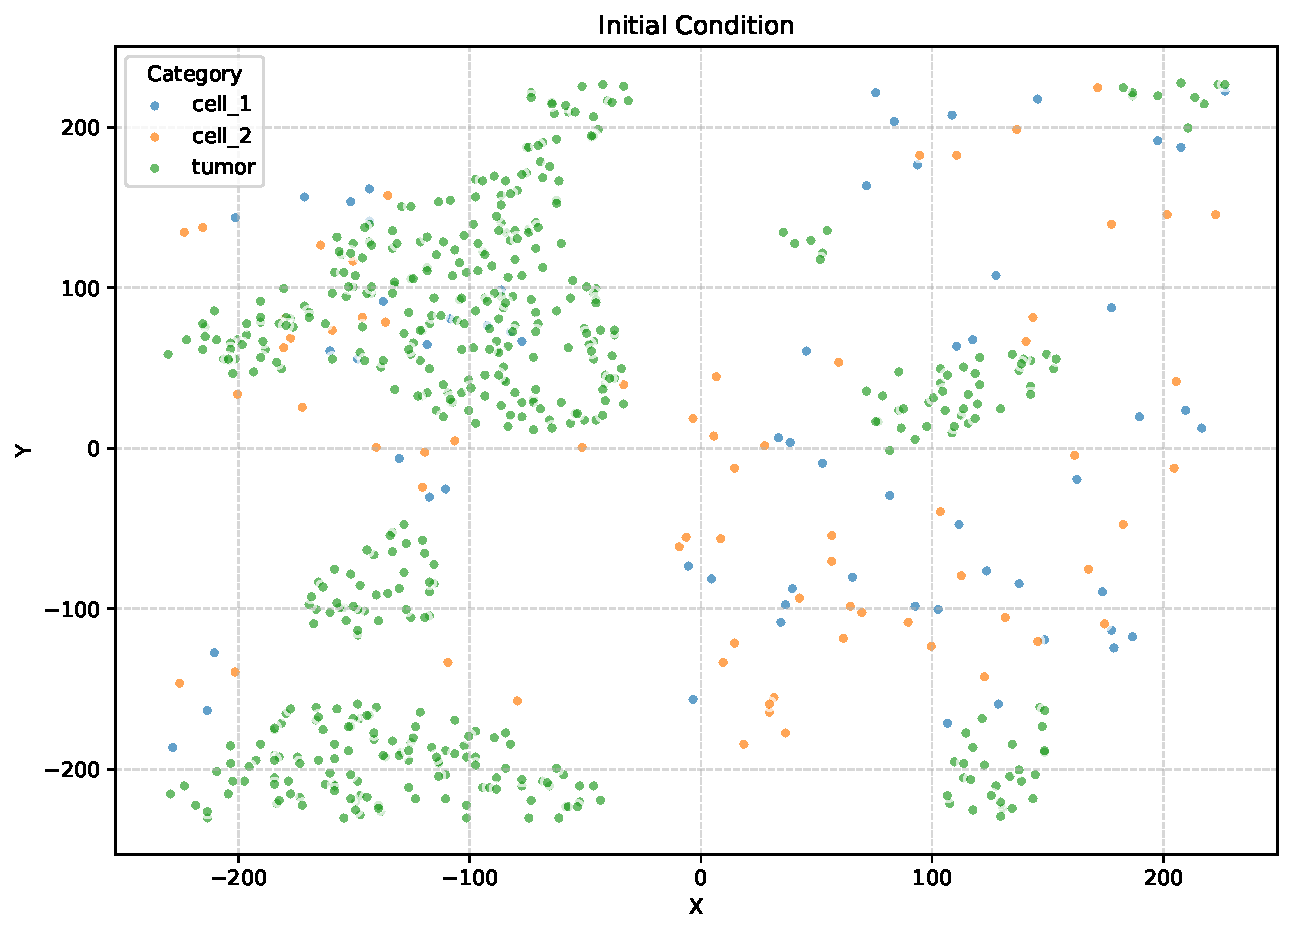
\includegraphics[width=\textwidth]{img/output_plot_0.pdf}
         \caption{Initial condition for seed 1, environment 1, episode 0}
    \end{subfigure}
    \hspace{5pt} % Fixed small gap instead of \hfill
    \begin{subfigure}[b]{0.4\textwidth}
         \centering
         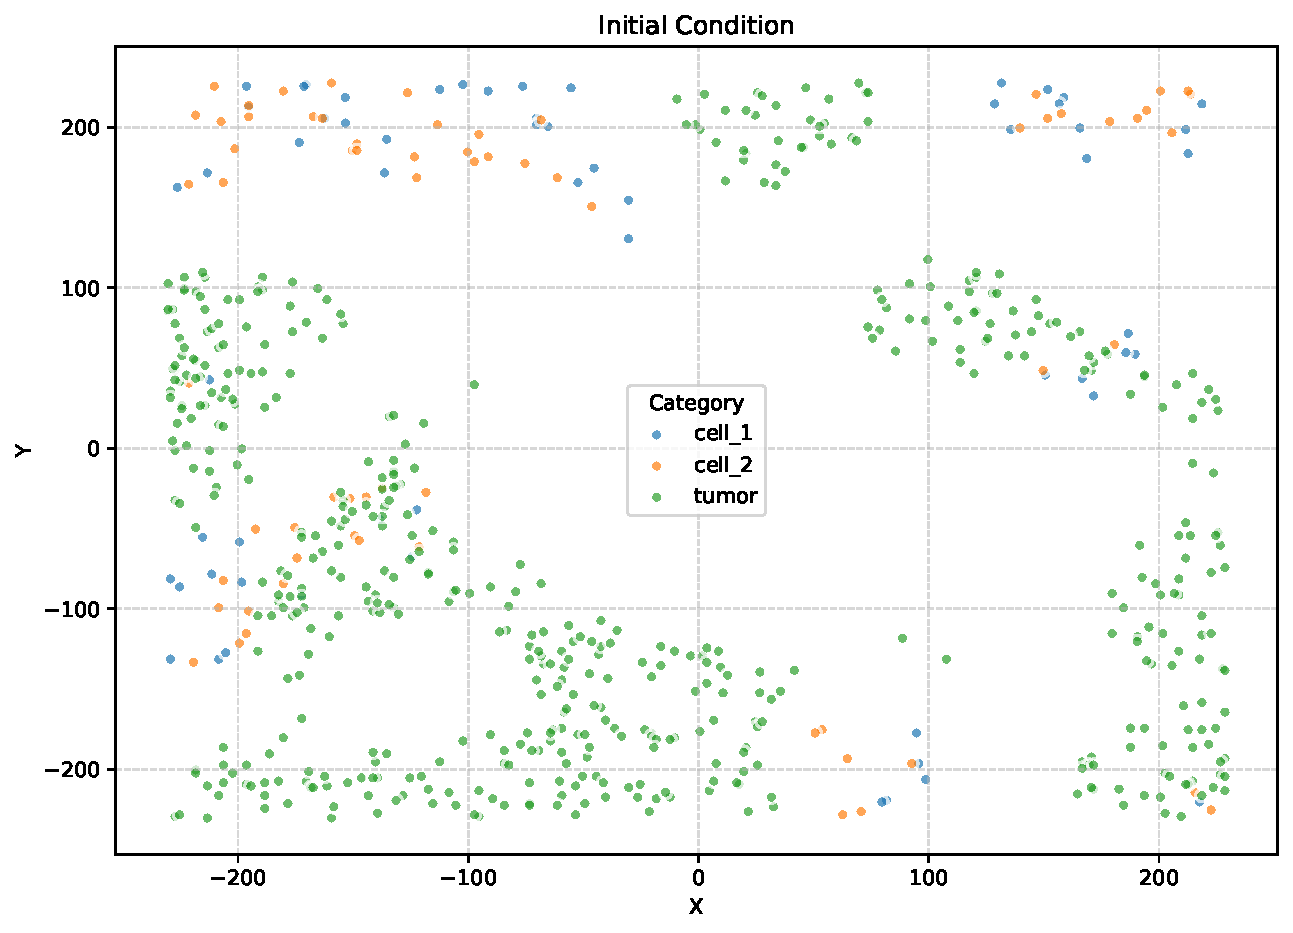
\includegraphics[width=\textwidth]{img/output_plot_1.pdf}
         \caption{Initial condition for seed 1, environment 1, episode 1}
    \end{subfigure}

    \vspace{8pt} % Space between rows

    % Second Row
    \begin{subfigure}[b]{0.4\textwidth}
         \centering
         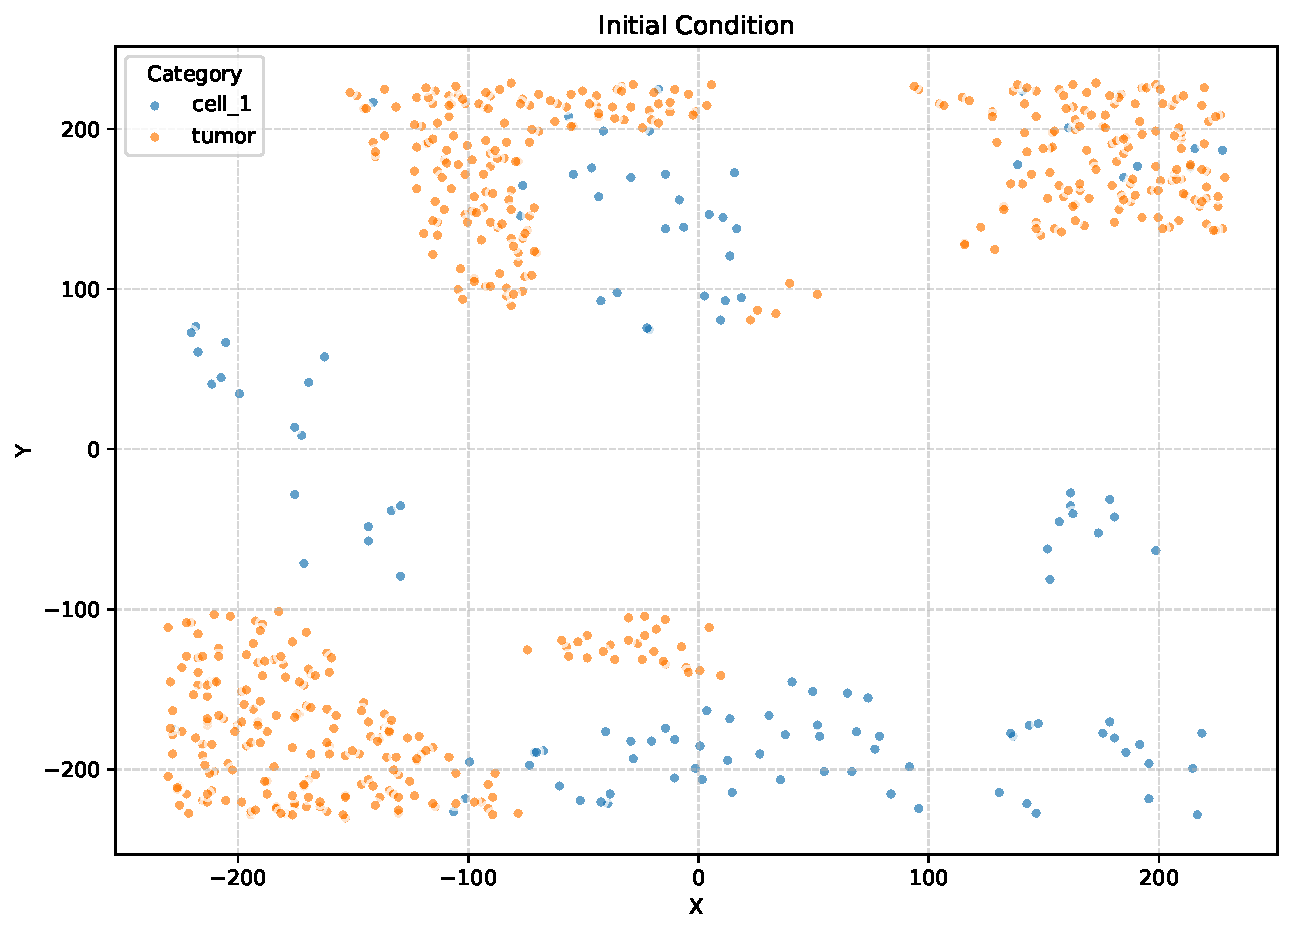
\includegraphics[width=\textwidth]{img/output_plot_5.pdf}
         \caption{Initial condition for seed 1, environment 1, episode 5}
    \end{subfigure}
    \hspace{5pt} % Fixed small gap instead of \hfill
    \begin{subfigure}[b]{0.4\textwidth}
         \centering
         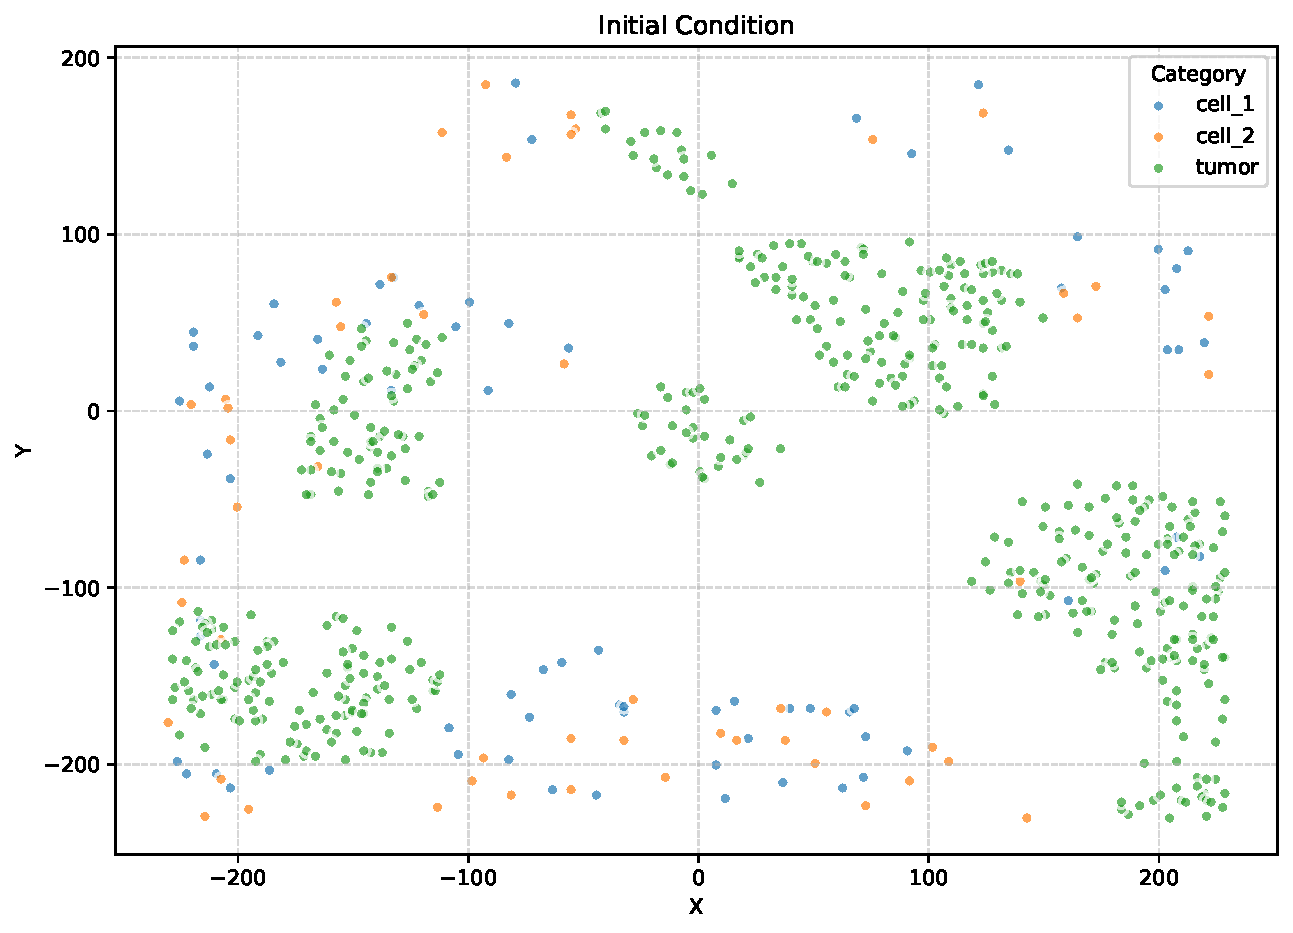
\includegraphics[width=\textwidth]{img/output_plot_7.pdf}
         \caption{Initial condition for seed 1, environment 1, episode 7}
    \end{subfigure}
    
    \caption{Four generated initial conditions.}
    \label{fig:four_plots}
\end{figure}

\newpage
\section{Neural architecture description}
\subsection{Neural Network Architecture}
\label{sec:neural_architecture}

We employ a modular neural architecture following an actor-critic paradigm, designed to accommodate heterogeneous observation modalities, including image-based, vector-based, and graph-structured state representations. A shared feature extraction module encodes observations into a common latent representation, which is then used by separate policy (actor) and value (critic) networks.

The feature extractor dynamically adapts to the observation type. Image-based inputs are processed through convolutional encoders, graph-structured inputs are handled by attention-based graph neural networks, and vector observations are passed directly without transformation. In all cases, the extracted features are flattened into a fixed-dimensional latent vector that serves as the input to both actor and critic networks.


\subsubsection{Convolutional Feature Extractors}

We have considered to use an IMPALA-style Convolutional Network for image-based inputs \cite{espeholt2018impala}.

\paragraph{IMPALA-style Convolutional Network.}
The first architecture is inspired by the IMPALA CNN design and consists of a stack of convolutional blocks. Each block comprises:
\begin{itemize}
    \item A $3 \times 3$ convolution,
    \item A $3 \times 3$ max-pooling operation with stride $2$,
    \item Two residual blocks with skip connections.
\end{itemize}

Each residual block applies two convolutional layers with Mish \cite{misra2019mish} nonlinearities and preserves the input through identity shortcuts. This structure promotes stable gradient flow and enables deep feature hierarchies.

\subsubsection{Graph-Based Feature Extraction}

For graph-structured observations, we employ a graph attention network (GAT) \cite{velickovic2017graph}. The extractor consists of two stacked GAT layers with multi-head attention in the first layer, followed by a single-head aggregation layer. Node embeddings are aggregated using global mean pooling to produce a fixed-dimensional graph-level representation. As activation function, we use Mish.




\subsubsection{Actor--Critic Networks}
\label{sec:actor_critic}

Both the actor and critic networks share a common architectural backbone following feature extraction. In each case, the extracted state representation is processed by a multilayer perceptron consisting of two fully connected layers of width $256$. Nonlinear activations are applied between layers (Mish for the critic and ReLU for the actor) .
\newpage
\section{Asynchronous SAC with Parallel Environments}

\subsection{Computational time}
We used a desktop machine (32 threads, 13th Gen Intel(R) Core(TM) i9-13900K) with an NVIDIA GeForce RTX 4090. The number of environments noted $N_{env}$ was 9, and 3 threads were used for a PhysiCell simulation and we  allocated the 5 left threads to the reinforcement learning algorithm. Empirically, we observed improved performance when using at least five threads for asynchronous SAC. Table~\ref{tab:state_space_means} reports the time required for different state space representations. Graph-based state spaces are the slowest, requiring more than two hours, whereas scalar state spaces are the fastest, taking less than one hour. Image-based state spaces exhibit intermediate performance, with a runtime of approximately one hour and thirty minutes.
\begin{table}[h!]
\centering
\caption{Mean Timestamp per State Space}
\label{tab:state_space_means}
\begin{tabular}{lr}
\hline
\textbf{State Space} & \textbf{Mean Timestamp (s)} \\ \hline
Random                   & 2893.75 \\ \hline
Scalars (cells)           & 3072.50 \\
Scalars (substrates)       & 3113.17 \\
Scalars (cells + substrates) & 3133.45 \\ \hline
Image (MC cells)            & 5160.60 \\
Image (MC substrates)       & 5175.52 \\
Image (MC cells + substrates)  & 5604.56 \\ \hline
Graph (kNN with k=3)                 & 8202.35 \\
Graph (Delaunay)         & 8525.22 \\
\hline
\end{tabular}
\end{table}\\
Table~\ref{tab:number_environments_means} illustrates the impact of varying the number of environments coupled with an appropriate choice of threads. The optimal number of threads depends on the complexity of the model: for more complex models, fewer environments per thread may be preferable to maximize efficiency. In our setup, using 9 environments with 3 threads per environment allowed us to collect 25000 steps in approximately 6 minutes. In contrast, running a single environment without vectorization would require more than 17 minutes. Thanks to vectorization, the time required to collect samples was effectively reduced by a factor of three, and this reduction could be further improved by increasing the total number of threads in order to increase the number of environments.\\
\begin{table}[h!]
\centering
\caption{The overall number of threads is $27$ Mean timestamp per number of environments for collecting 25000 steps}
\label{tab:number_environments_means}
\begin{tabular}{lccc}
\hline
\textbf{$N_{env}$} &
\textbf{$\mu$(s)} &
\textbf{$\sigma$(s)} &
\textbf{Threads per environment} \\
\hline
1  & 1059 & 11 & 27 \\ 
2  & 658  & 6  & 13 \\ 
3  & 529  & 3  & 9 \\ 
6  & 438  & 3  & 4 \\ 
9  & 363  & 5  & 3 \\
\hline
\end{tabular}
\end{table}
Table~\ref{tab:number_cells_time} demonstrates the impact of varying the number of tumor cells on the computational time required to collect 25,000 steps in 9 environments using 3 threads. It is clear that increasing the number of tumor cells significantly increases the computation time, with the largest configuration being substantially slower.

\begin{table}[h!]
\centering
\caption{Computational time for collecting 25,000 steps for 9 environments with 3 threads as a function of the number of tumor cells.}
\label{tab:number_cells_time}
\begin{tabular}{lcc}
\hline
\textbf{Number of tumor cells ($N_\mathrm{tumor}$)} & 
\textbf{Approximate time (min)} \\
\hline
512   & $\approx 6$    \\
1024  & $\approx 10$   \\
2048  & $\approx 30$   \\
4096  & $\approx 180$  \\
\hline
\end{tabular}
\end{table}
\newpage


\subsection{Hyperparameters}
\begin{table}[htbp]
\centering
\caption{Reinforcement learning algorithm hyperparameters.}
\label{tab:rl_hyperparameters}
\begin{tabular}{lll}
\hline
\textbf{Parameter} & \textbf{Symbol / Name} & \textbf{Value / Description} \\
\hline
Total training steps &
$T$ &
$2 \times 10^{5}$\\

Replay buffer size &
$|\mathcal{B}|$ &
$2 \times 10^{5}$ \\
Batch Size Multiplier &
$|\mathcal{BM}|$ &
\texttt{64} \\

Batch size &
$B$ &
$|\mathcal{BM}| \times N_{\text{env}}$ \\

Warm-up steps &
$T_{\text{start}}$/\texttt{learning\_starts} &
1e4 \\

Policy update frequency &
$f_{\pi}$ &
2 \\

Target network update frequency &
$f_{\text{target}}$ &
1 \\

Entropy autotuning &
-- &
Enabled (Boolean) \\

Entropy coefficient &
$\alpha$ &
0.05 \\
Target smoothing coefficient &
$\tau$ &
0.005 \\
Critic learning rate &
$\eta_Q$ &
$3 \times 10^{-4}$ \\
Policy learning rate &
$\eta_\pi$ &
$3 \times 10^{-4}$ \\
Discount factor &
$\gamma$ &
0.99 \\
Number of update loops per step &
$N_{\text{loops}}$ &
3 \\
\hline
\end{tabular}
\end{table}

\newpage
\subsection{Algorithm details}
\begin{algorithm}[H]
\caption{Asynchronous SAC with Parallel Environments}
\label{alg:async_sac}
\begin{algorithmic}[1]

\Require Simulator configuration $d_{\text{arg}}$, replay buffer size $|\mathcal{B}|$, learning rates, discount factor $\gamma$, target update rate $\tau$
\Ensure Trained SAC policy $\pi_\theta$

\State Initialize shared queues: \texttt{actor\_queue}, \texttt{sample\_queue}
\State Initialize stop signal \texttt{stop\_event}

\State Launch \textbf{Actor Process} (CPU)
\Statex \quad Initialize vectorized environments $\mathcal{E}_1, \dots, \mathcal{E}_N$
\Statex \quad Reset environments and obtain initial observations
\Statex \quad Initialize local policy $\pi_{\theta_a}$

\While{not \texttt{stop\_event}}
    \State Receive updated policy parameters from \texttt{actor\_queue} (if available)
    \If{total steps $< t_{\text{start}}$}
        \State Sample random actions
    \Else
        \State Sample actions from $\pi_{\theta_a}$
    \EndIf
    \State Step all environments in parallel
    \State Collect transitions $(s, a, r, s', d)$
    \State Send transition batches to \texttt{sample\_queue}
\EndWhile

\State Initialize \textbf{Learner Process} (GPU)
\State Initialize actor $\pi_\theta$, critics $Q_{\phi_1}, Q_{\phi_2}$
\State Initialize target critics $Q_{\phi_1'} \leftarrow Q_{\phi_1}$, $Q_{\phi_2'} \leftarrow Q_{\phi_2}$
\State Initialize replay buffer $\mathcal{D}$

\State Send initial policy parameters $\theta$ to actor via \texttt{actor\_queue}

\While{total samples $< T$}
    \State Drain transitions from \texttt{sample\_queue} into $\mathcal{D}$
    \If{$|\mathcal{D}| < \max(t_{\text{start}}, \text{batch size})$}
        \State Continue
    \EndIf

    \For{$N_{loops}$}
        \For{each gradient update step}
            \State Sample minibatch from $\mathcal{D}$
            \State Compute SAC target:
            \[
            y = r + \gamma (1-d) \left[
            \min(Q_{\phi_1'}, Q_{\phi_2'}) - \alpha \log \pi_\theta(a'|s')
            \right]
            \]
            \State Update critics $Q_{\phi_1}, Q_{\phi_2}$
            \State Update actor $\pi_\theta$
            \State Update entropy coefficient $\alpha$ (if enabled)
            \State Soft-update targets:
            \[
            \phi' \leftarrow \tau \phi + (1-\tau)\phi'
            \]
        \EndFor
    \EndFor

    \If{policy update interval reached}
        \State Send updated policy parameters to actor
    \EndIf
\EndWhile

\end{algorithmic}
\end{algorithm}
\newpage
\subsection{Bootstrapped Results}
The results are derived from the same set of raw learning curves obtained from five different random seeds. Given these five raw curves, we generate 256 bootstrap replicates by resampling the seed dimension with replacement. For each bootstrap replicate, a mean learning curve is computed across the resampled seeds and subsequently smoothed using an exponentially weighted moving average (EWMA) with $\alpha = 0.01$. The reported mean corresponds to the EWMA-smoothed average across the original seeds, while confidence intervals are estimated from the empirical distribution of the bootstrapped EWMA curves.
\begin{figure}[h!]%
\centering
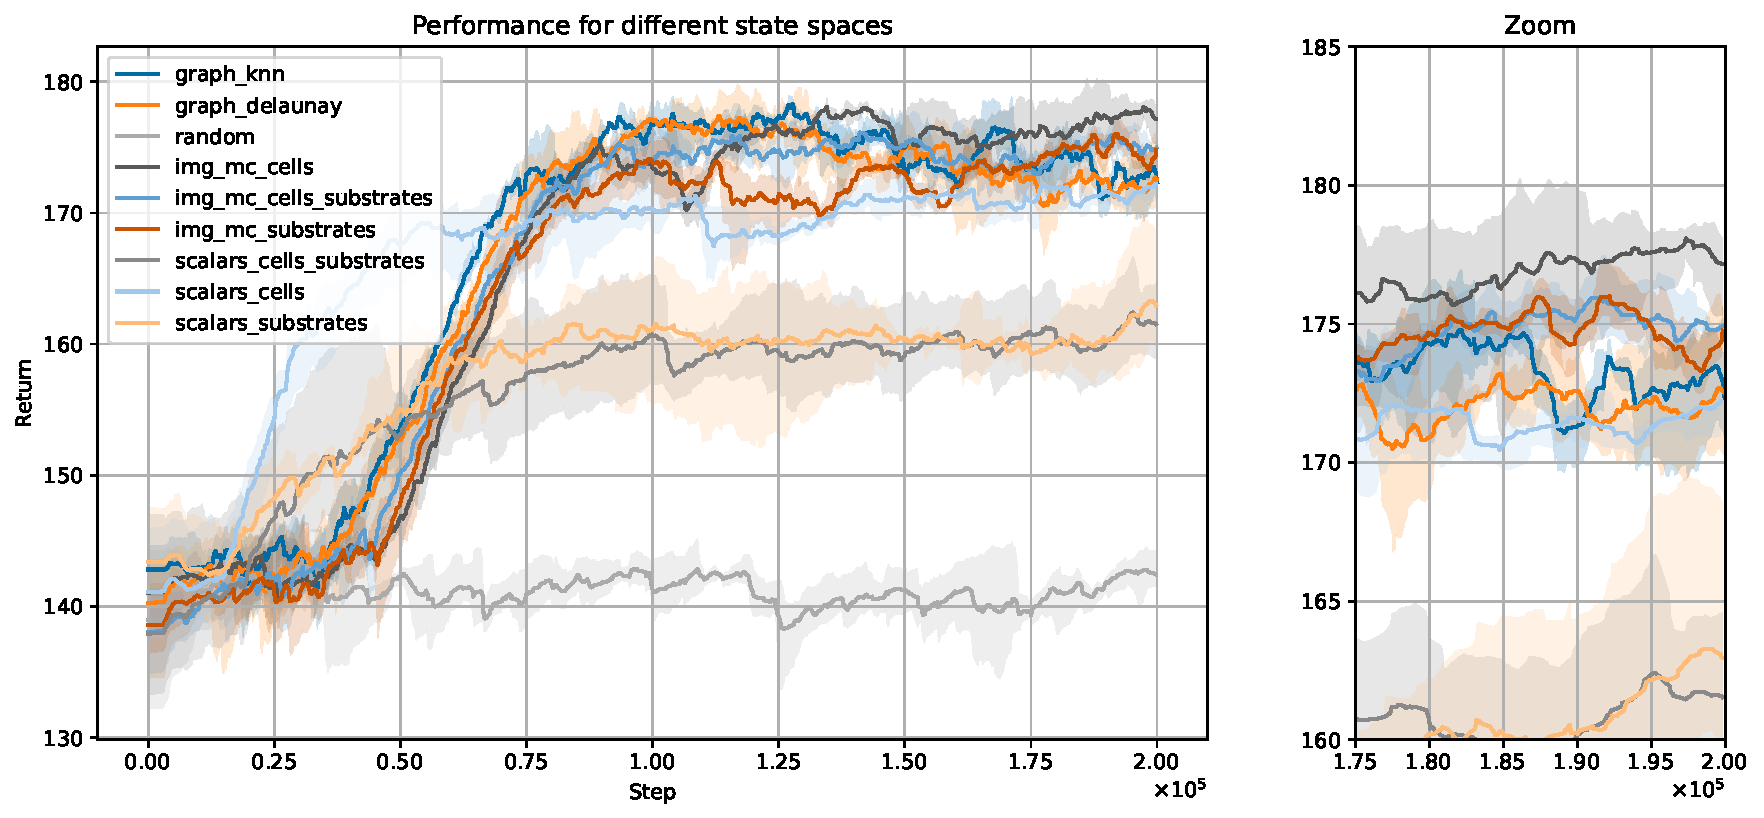
\includegraphics[width=1.0\textwidth]{img/bootstrap_performance.pdf}
\caption{Performance bootstrapped for different state spaces X-axis represents the number of steps while Y-axis represents the return across 5 different seeds.}
\label{bootstrap_performance}
\end{figure}

\begin{table}[h!]
\centering
\begin{tabular}{lccc}
\hline
\textbf{Observation type} &
\textbf{$\mu$} &
\textbf{CI low} ($2.5\%$) &
\textbf{CI high ($97.5\%$)} \\
\hline
Random & 142.46 & 141.42 & 144.27 \\
\hline
Scalars (cells) & 172.2 & 170.54 & 174.28 \\
Scalars (substrates) & 162.96 & 159.68 & 168.55 \\
Scalars (cells + substrates) & 160.50 & 156.56  & 164.6 \\
\hline
Image (Multi-Channel cells) & 177.17 & 176.25 & 178.09\\
Image (Multi-Channel substrates) & 174.78 & 174.18 & 175.63 \\
Image (Multi-Channel cells + substrates) & 174.95 & 174.77 & 175.21 \\
\hline
Graph (kNN with k=3) & 172.3 & 170.82 & 174.07\\
Graph (Delaunay) & 172.52 & 170.48 & 175.31\\
\hline
\end{tabular}
\caption{Mean performance ($\mu$) with confidence interval bounds for different observation types.}
\label{tab:observation_ci}
\end{table}
We quantitatively observe the same trends in the corresponding results, consistent with the previous Figure ~\ref{performance}.

%\bibliographystyle{plain}
%\bibliography{reference}


%USE THE BELOW OPTIONS IN CASE YOU NEED AUTHOR YEAR FORMAT.



\end{document}

d_{\text{drugs},t} = \frac{1}{2T}\sum_{i=1}^{2}d_{i,t}\\
\frac{c_{t}-c_{t-1}}{c_{\text{init}}}=c_{\text{norm},t}\\
R(t) = - (\alpha c_{\text{norm},t} + (1-\alpha)d_{\text{drugs},t})\\
\text{cumulative return refers to} \sum_{t=1}^{T}R(t)
